%!TEX root = ../../Master.tex
\section{Use Cases}

Udviklingen af løsningen er sket på baggrund at de forudgående analyser, samt mange diskussioner og overvejelser omkring mulige vinkler hvorpå problemet kan gribes an. Som en del af processen blev der lavet use cases. 

Det gøres for at udpensle sandsynlige arbejdsmønstre i den tiltænkte løsning og for at normalisere ideer om interaktion med systemet.

Der er mange forskellige tilgange til use cases, men de tager udgangspunkt i det samme princip. I denne rapport er use cases lavet efter kapitel 17 i \enquote{Agile Principles, Patterns, and Practices in C\#} \cite{martin2006agile}. Denne bog er valgt fordi den har en simpel tilgang til use cases. Her følger en beskrivelse af use cases som præsenteret i \cite{martin2006agile}.

En use case er i simpleste forstand en række af trin, der bliver udført mellem en person, kaldt aktøren, og et system. Traditionelt er en use case skrevet meget udførlig, men \cite{martin2006agile} mener at use cases handler om at skrive det primære forløb af trin. Ved at gøre det simpelt sikres, at der ikke bliver brugt tid på at diskutere punkter, der ikke er vigtige. 

Trinene til use cases tager udgangspunkt i et problemfrit forløb. Dertil kan skrives et alternativt forløb til sandsynlige afvigelser fra den problemfrie brug.

\subsection{Use Case Diagram}
For at visualisere et systems use case, opsættes det i et use case diagram. Dette diagram visualiserer de aktuelle aktøre samt systemet og dets funktioner. I diagrammet er systemet repræsenteret som en aflang rektangel, med dets use cases repræsenteret af de ovale cirkler. Alt inden for rektanglet er systemet som skal udvikles. Uden for systemet ses aktørerne samt hvilke use cases de kan interagere med som er repræsenteret af linjerne. En af fordelene ved at lave dette diagram, er at der skabes et overblik, samt en bedre forståelse af hvilke aktørere der interagere med hvilke use cases. Diagrammet kaldes ofte for et system boundary diagram fordi det effektivt visualisere et systems grænser. På \cref{fig:usecase} ses et use case diagram for LOBOP.
\begin{figure}[h]
  \centering
    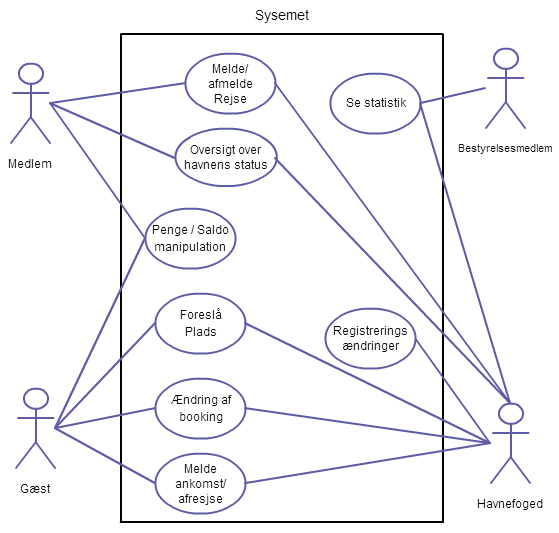
\includegraphics[width=\textwidth]{use_case_diagram.png}
  \caption{LOBOP System boundary diagram}
  \label{fig:usecase}
\end{figure}


\section{Vores Specifikke Use Cases}
Her følger use cases, der er inddelt i fire kategorier, alt efter hvorvidt den pågældende use case tager udgangspunkt fra enten et medlem, en gæst, havnefogeden eller en fjerde. Når der skrives at \enquote{systemet melder}, i sammenhæng med en plads, hentydes der til den visuelle repræsentation af pladsens tilgængelighed, \cref{sub:gaster_havnefogeden}.
\frnote{der skal mere tekst}

\subsection{Medlemmer}  
  \begin{enumerate}

    \item{\bf{Medlem forlader sin plads i mere end 24 timer}}
      \begin{enumerate}
        \item Medlemmet melder til systemet et gyldigt tidspunkt for afrejse og hjemkomst.
        \item Systemet melder til medlemmet at rejsen er registreret.
        \item Systemet venter til efter tidspunktet for afrejse.
        \item Når pladsen tømmes, melder systemet at pladsen er fri.
      \end{enumerate}

    \paragraph{Alternativ: medlem melder ikke afrejse til systemet}
      \begin{enumerate}
        \item Systemet underretter havnefogeden om at en medlemsbåd har været væk fra havnen i mere end 24 timer.
      \end{enumerate}

    % Brian mener at vi skal Undgå simpel input validering i use case
    %\paragraph{Alternativ: rejsens dato er ikke gyldig}
    %  \begin{enumerate}
    %    \item Systemet melder at indtastet dato ikke er gyldig.
    %    \item Systemet anmoder om nyt tidspunkt.
    %  \end{enumerate}

    \paragraph{Alternativ: medlem afrejser ikke på meldte tidspunkt}
      \begin{enumerate}
        \item Systemet underetter både havnefogeden samt medlemmet om uoverensstemmelsen.
      \end{enumerate}


    \item{\bf{Medlem vender tilbage til sin plads efter minimum 24 timers afrejse}}
      \begin{enumerate}
        \item Systemet melder at pladsen er optaget.
      \end{enumerate}


    \item{\bf{Medlem vender ikke tilbage til sin plads på meldte tidspunkt}}
      \begin{enumerate}
        \item Systemet melder uoverensstemmelsen til havnefogeden.
      \end{enumerate}


    \item{\bf{Medlemmet ønsker at annullere en allerede anmeldt rejse}}
      \begin{enumerate}
        \item Medlemmet vælger den pågældende rejse fra listen over registrerede rejser.
        \item Medlemmet annullerer rejsen.
        \item Systemet melder tilbage at rejsen er annulleret.
      \end{enumerate}


\subsection{Gæster}


    \item{\bf{Gæst er ankommet til havnen, og vil leje en plads}}
      \begin{enumerate}
        \item Gæsten vælger i system brugergrænsefladen, den plads han har fundet til sin båd.
        \item Gæsten betaler for pladsen.
        \item Systemet melder at pladsen nu er optaget.
        \item Gæsten får udleveret et chipkort og en kvittering.
        \item Systemet melder til havnefogeden at der er nye ankomne.
      \end{enumerate}

    \paragraph{Alternativ: Gæsten finder ikke selv en plads}
      \begin{enumerate}
        \item Ny gæst melder til systemet, hvor lang tid han vil ligge til.
        \item Systemet returnerer en liste over pladser som vil passe hans behov.
        \item Systemet videresender gæsten til betaling.

      \end{enumerate}

    \item{\bf{Gæst vil se informationer om plads og betaling}}
      \begin{enumerate}
        \item Gæst indsætter chipkort i automat.
        \item Systemet viser informationer vedrørende gæsten.
      \end{enumerate}

    \paragraph{Alternativ: Chipkort er bortkommet}
      \begin{enumerate}
        \item Gæster melder til systemet at chipkort er bortkommet.
        \item Systemet henviser gæsten til havnefogeden.
      \end{enumerate}


    \item{\bf{Gæst forlader havnen på eller før anmeldte afrejse tidspunkt}}
      \begin{enumerate}
        \item Gæst aflever chipkort og får udleveret en kvittering.
        \item Gæst får returneret berettiget kapital.
      \end{enumerate}

    \paragraph{Alternativ: Gæst bliver liggende i havnen efter det anmeldte afrejse tidspunkt}
      \begin{enumerate}
        \item Systemet melder uoverensstemmelsen til havnefogeden.
        \item Chipkortet deaktiveres.
        \item Ved efterfølgende forsøg på brug af chipkort, henvendes der til havnefogeden.
      \end{enumerate}


    \item{\bf{Gæst vil forlænge ophold}}
      \begin{enumerate}
        \item Gæst indsætter chipkort i automat.
        \item Gæst melder ønskede ny afrejse dato til systemet.
        \item Systemet melder at den nye dato er registreret.
      \end{enumerate}

    \paragraph{Alternativ: Nye afrejse dato overlapper med medlemshjemkomst}
      \begin{enumerate}
        \item Systemet melder at datoerne overlapper, og foreslår ny plads.
      \end{enumerate}

\subsection{Havnefoged}
    \item{\bf{Havnefogeden registrerer et medlemmets hjemkost}}
      \begin{enumerate}
        \item Medlem meddeler tidlig hjemkomst til havnefogeden, for eksempel via telefon, mail eller lignende.
        \item Havnefogeden indtaster (ny) dato i systemet.
        \item Systemet returnere at datoen er accepteret
      \end{enumerate}
  
    \paragraph{Alternativ: En gæst har lejet pladsen for en længere periode.}
      \begin{enumerate}
        \item Systemet foreslår en ny plads til gæsten.
        \item Havnefogeden snakker med gæsten.
      \end{enumerate}

    \item{\bf{Havnefogeden vil gerne se hvilke pladser der er ledige}}
      \begin{enumerate}
        \item Havnefogeden åbner overbliksfunktionen i programmet.
        \item Havnefogeden kan nu se på et kort over havnen, hvilke pladser der er ledige.
      \end{enumerate}

    \item{\bf{Havnefogeden vil gerne se hvilke nye gæster der er ankommet indenfor et tidsrum}}
      \begin{enumerate}
        \item Havnefogeden åbner gæster funktionen i programmet.
        \item Havnefogeden vælger det ønskede tidsrum.
        \item Programmet viser nye ankomne gæster fra det specificerede tidsrum.
      \end{enumerate}

    \item{\bf{Havnefogeden vil gerne se hvilke pladser der endnu ikke er betalt for}}
      \begin{enumerate}
        \item Havnefogeden åbner gæster funktionen i programmet.
        \item Havnefogeden åbner ubetalte pladser.
        \item Programmet præsenterer listen af pladser, der endnu ikke er betalt for. Tiden for hvor lang tid pladsen har været ubetalt vises også.
      \end{enumerate}

    \item{\bf{Havnefogeden vil gerne se hvornår et medlem vender tilbage til medlemmets plads}}
      \begin{enumerate}
        \item Havnefogeden åbner medlems funktionen i programmet.
        \item Havnefogeden skriver i søgefeltet medlemmets navn eller medlemsnummer.
        \item Programmet præsenterer en liste over matchende medlemmer.
        \item Havnefogeden vælger det søgte medlem.
        \item Programmet viser alle kendte detaljer om medlemmet, herunder hvornår medlemmet forventes tilbage.
      \end{enumerate}

    \item{\bf{Havnefogeden bliver advaret af en fejl ved en stander}}
      \begin{enumerate}
        \item Uventet fejl opstår ved en stander på havnen, eller personen ved standeren trykker på hjælp.
        \item Havnefogeden får besked om dette.
      \end{enumerate}

\subsection{Andre}

    \item{\bf{Automatisk arrangementsforslag}}
      \begin{enumerate}
        \item Systemet melder på baggrund af aktiviteten i havnen, at det ville være en god dag for et arrangement.
        \item Et medlem af klubben ser denne melding, og foreslår et arrangement.
      \end{enumerate}

    \item{\bf{Automatisk medlemstjek}}
      \begin{enumerate}
        \item Systemet registrerer uoverensstemmelse med angivet rejseplan.
        \item Systemet notificerer havnefogeden omkring overensstemmelsen.
      \end{enumerate}

    \item{\bf{Bestyrelsen eller havnefogeden vil se statistik over aktivitet i havnen}}
      \begin{enumerate}
        \item Statistik funktionen åbnes og viser de ønskede statistikker.
      \end{enumerate}

  \end{enumerate}
